\documentclass[border=10pt]{standalone}
\usepackage{tikz}\usepackage{amsmath}\usetikzlibrary{matrix,arrows.meta}
\begin{document}
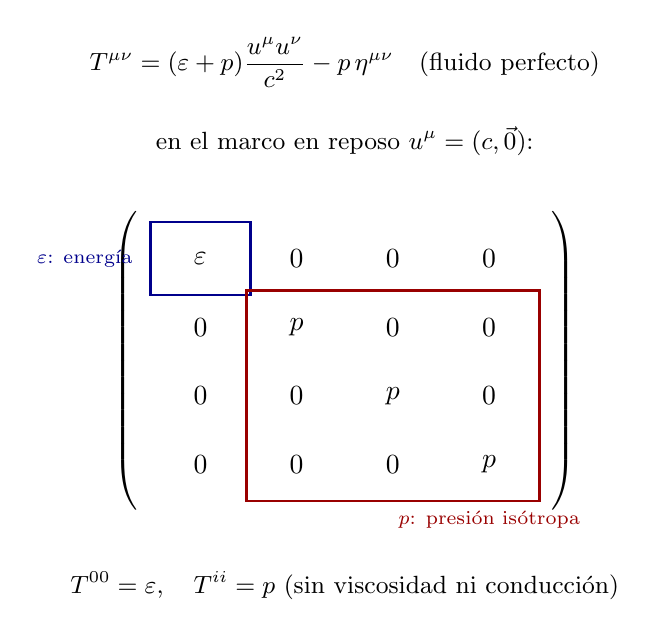
\begin{tikzpicture}[line width=0.8pt]
  \node at (0,3.1){\small $T^{\mu\nu}=(\varepsilon+p)\dfrac{u^\mu u^\nu}{c^2}-p\,\eta^{\mu\nu}$\quad(fluido perfecto)};
  \node at (0,2.1){\small en el marco en reposo $u^\mu=(c,\vec 0)$:};
  \matrix (T) [matrix of math nodes, left delimiter={(}, right delimiter={)},
     nodes={minimum width=1.25cm,minimum height=0.9cm,anchor=center},
     row sep=-\pgflinewidth, column sep=-\pgflinewidth] at (0,-0.7){
    \varepsilon & 0 & 0 & 0 \\
    0 & p & 0 & 0 \\
    0 & 0 & p & 0 \\
    0 & 0 & 0 & p \\
  };
  \draw[blue!55!black,line width=1pt] (T-1-1.north west) rectangle (T-1-1.south east);
  \draw[red!60!black,line width=1pt] (T-2-2.north west) rectangle (T-4-4.south east);
  \node[blue!55!black,anchor=east] at (T-1-1.west){\scriptsize $\varepsilon$: energía\ \ };
  \node[red!60!black,anchor=north,align=center] at (T-4-4.south){\scriptsize $p$: presión isótropa};
  \node at (0,-3.55){\small $T^{00}=\varepsilon,\quad T^{ii}=p$ (sin viscosidad ni conducción)};
\end{tikzpicture}
\end{document}
